\documentclass[tikz,border=10pt]{standalone}
\usepackage{tikz}
\usepackage{xcolor}
\usepackage{amsmath}
\usepackage{amssymb}

\usetikzlibrary{
    shapes.geometric,
    shapes.arrows,
    shapes.multipart,
    positioning,
    fit,
    calc,
    backgrounds,
    arrows.meta,
    decorations.pathreplacing,
    decorations.pathmorphing,
    shadows.blur,
    patterns
}

% Define custom colors
\definecolor{inputblue}{RGB}{41, 128, 185}
\definecolor{hyperbolicred}{RGB}{231, 76, 60}
\definecolor{hyperbolicpink}{RGB}{255, 118, 117}
\definecolor{agentgreen}{RGB}{46, 204, 113}
\definecolor{agentdarkgreen}{RGB}{39, 174, 96}
\definecolor{hybridgold}{RGB}{241, 196, 15}
\definecolor{hybridyellow}{RGB}{255, 215, 0}
\definecolor{adversarialorange}{RGB}{230, 126, 34}
\definecolor{utilgray}{RGB}{149, 165, 166}
\definecolor{darkgray}{RGB}{52, 73, 94}

% Define styles
\tikzset{
    % Box styles
    inputbox/.style={
        rectangle,
        rounded corners=3pt,
        minimum width=3cm,
        minimum height=0.8cm,
        text centered,
        draw=inputblue,
        fill=inputblue!20,
        line width=1pt,
        font=\small\sffamily,
        blur shadow={shadow blur steps=5}
    },
    hyperbox/.style={
        rectangle,
        rounded corners=3pt,
        minimum width=2.2cm,
        minimum height=0.65cm,
        text centered,
        draw=hyperbolicred,
        fill=hyperbolicpink!15,
        line width=0.8pt,
        font=\scriptsize\sffamily,
        blur shadow={shadow blur steps=3}
    },
    agentbox/.style={
        rectangle,
        rounded corners=3pt,
        minimum width=2.2cm,
        minimum height=0.65cm,
        text centered,
        draw=agentdarkgreen,
        fill=agentgreen!15,
        line width=0.8pt,
        font=\scriptsize\sffamily,
        blur shadow={shadow blur steps=3}
    },
    hybridbox/.style={
        rectangle,
        rounded corners=3pt,
        minimum width=2cm,
        minimum height=0.65cm,
        text centered,
        draw=hybridgold,
        fill=hybridyellow!15,
        line width=0.8pt,
        font=\scriptsize\sffamily,
        blur shadow={shadow blur steps=3}
    },
    adversarialbox/.style={
        rectangle,
        rounded corners=3pt,
        minimum width=2.2cm,
        minimum height=0.65cm,
        text centered,
        draw=adversarialorange,
        fill=adversarialorange!15,
        line width=0.8pt,
        font=\scriptsize\sffamily,
        blur shadow={shadow blur steps=3}
    },
    utilbox/.style={
        rectangle,
        rounded corners=2pt,
        minimum width=1.8cm,
        minimum height=0.5cm,
        text centered,
        draw=utilgray,
        fill=utilgray!10,
        line width=0.6pt,
        font=\tiny\sffamily
    },
    % Arrow styles
    hyperarrow/.style={
        -Stealth,
        line width=1.2pt,
        color=hyperbolicred
    },
    agentarrow/.style={
        -Stealth,
        line width=1.2pt,
        color=agentgreen
    },
    hybridarrow/.style={
        -Stealth,
        line width=1.2pt,
        color=hybridgold
    },
    adversarialarrow/.style={
        -Stealth,
        line width=1.2pt,
        color=adversarialorange
    },
    convergearrow/.style={
        -Stealth,
        line width=1.5pt,
        color=darkgray
    },
    % Label styles
    metriclabel/.style={
        font=\tiny\ttfamily,
        text=darkgray
    },
    sectionlabel/.style={
        font=\small\bfseries\sffamily,
        text=darkgray
    }
}

\begin{document}
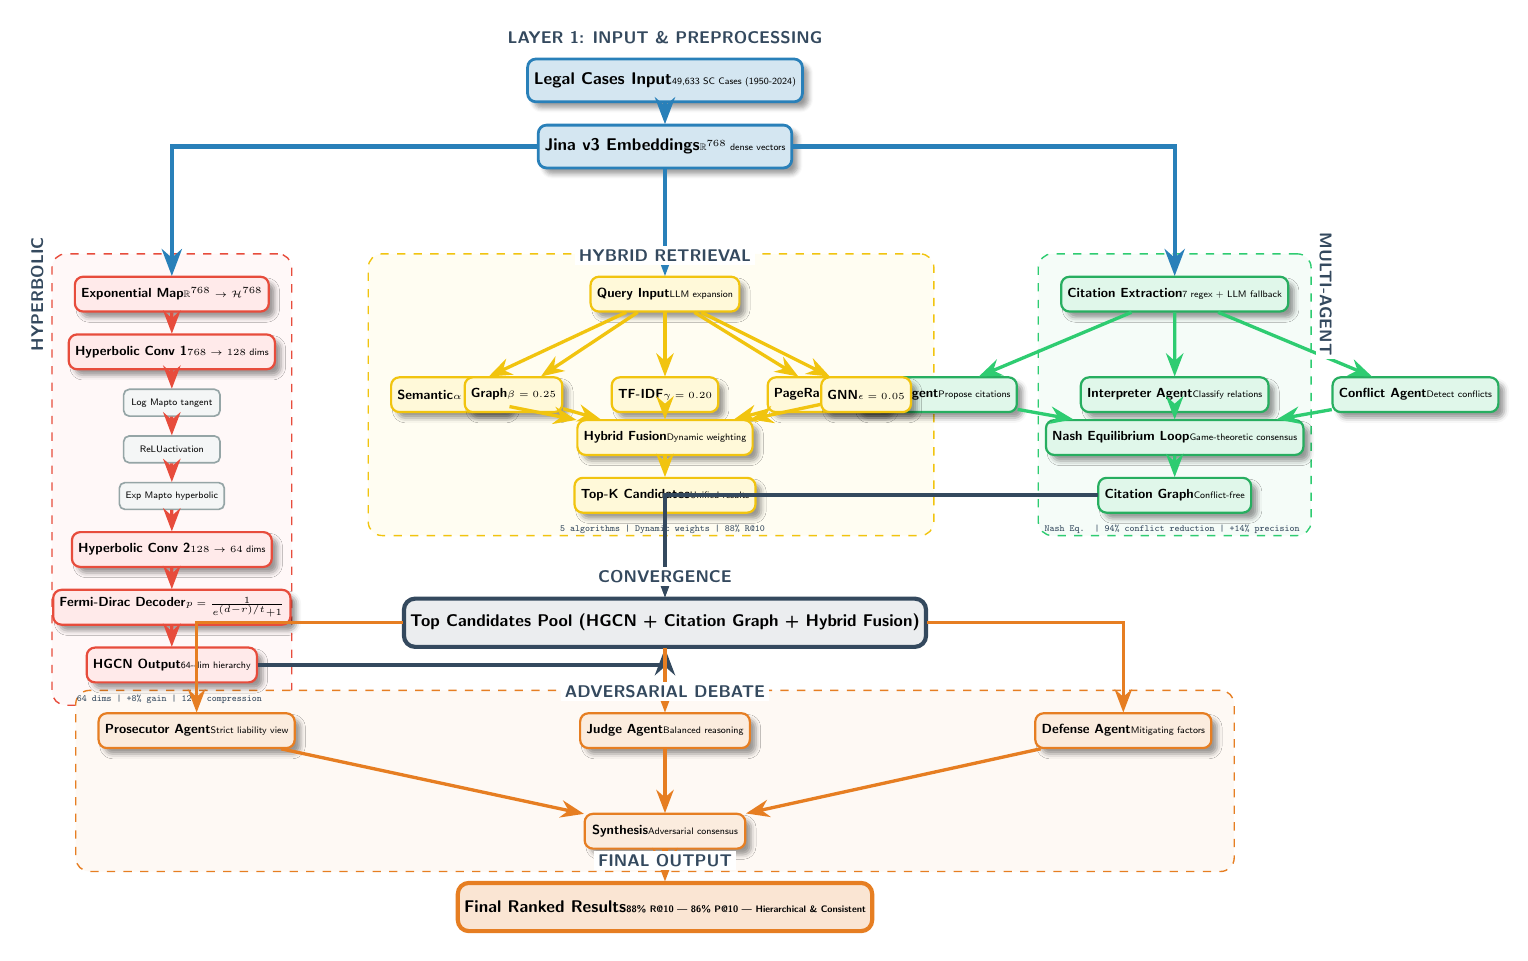
\begin{tikzpicture}[
    node distance=0.5cm and 1.5cm,
    >=Stealth,
    scale=0.68,
    every node/.style={transform shape}
]

% ============ LAYER 1: INPUT & PREPROCESSING ============
\node[inputbox, minimum width=4cm] (input) at (0, 0) {
    \textbf{Legal Cases Input}\\
    \tiny 49,633 SC Cases (1950-2024)
};

\node[inputbox, below=0.4cm of input] (jina) {
    \textbf{Jina v3 Embeddings}\\
    \tiny $\mathbb{R}^{768}$ dense vectors
};

\draw[inputblue, line width=1.5pt, -Stealth] (input) -- (jina);

% ============ LAYER 2: THREE PARALLEL BRANCHES ============

% -------- BRANCH 1: HYPERBOLIC (LEFT) --------
\node[hyperbox, below left=2cm and 5cm of jina] (exp1) {
    \textbf{Exponential Map}\\
    \tiny $\mathbb{R}^{768} \to \mathcal{H}^{768}$
};

\node[hyperbox, below=0.4cm of exp1] (hconv1) {
    \textbf{Hyperbolic Conv 1}\\
    \tiny $768 \to 128$ dims
};

\node[utilbox, below=0.35cm of hconv1] (log1) {
    Log Map\\
    \tiny to tangent
};

\node[utilbox, below=0.35cm of log1] (relu1) {
    ReLU\\
    \tiny activation
};

\node[utilbox, below=0.35cm of relu1] (exp2) {
    Exp Map\\
    \tiny to hyperbolic
};

\node[hyperbox, below=0.4cm of exp2] (hconv2) {
    \textbf{Hyperbolic Conv 2}\\
    \tiny $128 \to 64$ dims
};

\node[hyperbox, below=0.4cm of hconv2] (fermi) {
    \textbf{Fermi-Dirac Decoder}\\
    \tiny $p = \frac{1}{e^{(d-r)/t} + 1}$
};

\node[hyperbox, below=0.4cm of fermi] (hgcn) {
    \textbf{HGCN Output}\\
    \tiny 64-dim hierarchy
};

% Hyperbolic connections
\draw[hyperarrow] (exp1) -- (hconv1);
\draw[hyperarrow] (hconv1) -- (log1);
\draw[hyperarrow] (log1) -- (relu1);
\draw[hyperarrow] (relu1) -- (exp2);
\draw[hyperarrow] (exp2) -- (hconv2);
\draw[hyperarrow] (hconv2) -- (fermi);
\draw[hyperarrow] (fermi) -- (hgcn);

% Metrics label
\node[metriclabel, below=0.1cm of hgcn, align=center] {
    64 dims | +8\% gain | 12$\times$ compression
};

% -------- BRANCH 2: MULTI-AGENT (RIGHT) --------
\node[agentbox, below right=2cm and 5cm of jina] (citextract) {
    \textbf{Citation Extraction}\\
    \tiny 7 regex + LLM fallback
};

\node[agentbox, below left=1.2cm and 0.8cm of citextract] (linker) {
    \textbf{Linker Agent}\\
    \tiny Propose citations
};

\node[agentbox, below=1.2cm of citextract] (interpreter) {
    \textbf{Interpreter Agent}\\
    \tiny Classify relations
};

\node[agentbox, below right=1.2cm and 0.8cm of citextract] (conflict) {
    \textbf{Conflict Agent}\\
    \tiny Detect conflicts
};

% Three agents connections
\draw[agentarrow] (citextract) -- (linker);
\draw[agentarrow] (citextract) -- (interpreter);
\draw[agentarrow] (citextract) -- (conflict);

\node[agentbox, below=2cm of citextract, minimum width=2.8cm] (nash) {
    \textbf{Nash Equilibrium Loop}\\
    \tiny Game-theoretic consensus
};

\draw[agentarrow] (linker) -- (nash);
\draw[agentarrow] (interpreter) -- (nash);
\draw[agentarrow] (conflict) -- (nash);

\node[agentbox, below=0.4cm of nash] (citgraph) {
    \textbf{Citation Graph}\\
    \tiny Conflict-free
};

\draw[agentarrow] (nash) -- (citgraph);

% Metrics label
\node[metriclabel, below=0.1cm of citgraph, align=center] {
    Nash Eq. | 94\% conflict reduction | +14\% precision
};

% -------- BRANCH 3: HYBRID RETRIEVAL (CENTER) --------
\node[hybridbox, below=2cm of jina] (query) {
    \textbf{Query Input}\\
    \tiny LLM expansion
};

% Five retrieval algorithms
\node[hybridbox, below left=1.2cm and 1.5cm of query, minimum width=1.6cm] (semantic) {
    \textbf{Semantic}\\
    \tiny $\alpha=0.35$
};

\node[hybridbox, below left=1.2cm and 0.5cm of query, minimum width=1.6cm] (graph) {
    \textbf{Graph}\\
    \tiny $\beta=0.25$
};

\node[hybridbox, below=1.2cm of query, minimum width=1.6cm] (tfidf) {
    \textbf{TF-IDF}\\
    \tiny $\gamma=0.20$
};

\node[hybridbox, below right=1.2cm and 0.5cm of query, minimum width=1.6cm] (pagerank) {
    \textbf{PageRank}\\
    \tiny $\delta=0.15$
};

\node[hybridbox, below right=1.2cm and 1.5cm of query, minimum width=1.6cm] (gnn) {
    \textbf{GNN}\\
    \tiny $\epsilon=0.05$
};

% Connections to algorithms
\draw[hybridarrow] (query) -- (semantic);
\draw[hybridarrow] (query) -- (graph);
\draw[hybridarrow] (query) -- (tfidf);
\draw[hybridarrow] (query) -- (pagerank);
\draw[hybridarrow] (query) -- (gnn);

\node[hybridbox, below=2cm of query, minimum width=2.8cm] (fusion) {
    \textbf{Hybrid Fusion}\\
    \tiny Dynamic weighting
};

\draw[hybridarrow] (semantic) -- (fusion);
\draw[hybridarrow] (graph) -- (fusion);
\draw[hybridarrow] (tfidf) -- (fusion);
\draw[hybridarrow] (pagerank) -- (fusion);
\draw[hybridarrow] (gnn) -- (fusion);

\node[hybridbox, below=0.4cm of fusion] (topk) {
    \textbf{Top-K Candidates}\\
    \tiny Unified results
};

\draw[hybridarrow] (fusion) -- (topk);

% Metrics label
\node[metriclabel, below=0.1cm of topk, align=center] {
    5 algorithms | Dynamic weights | 88\% R@10
};

% ============ CONVERGENCE TO CANDIDATES ============
\node[rectangle, rounded corners=4pt, minimum width=8cm, minimum height=0.9cm,
      draw=darkgray, fill=darkgray!10, line width=1.5pt,
      below=2.5cm of jina, xshift=0cm, yshift=-5.5cm,
      font=\small\sffamily\bfseries] (candidates) {
    Top Candidates Pool (HGCN + Citation Graph + Hybrid Fusion)
};

% Convergence arrows
\draw[convergearrow] (hgcn) -| (candidates);
\draw[convergearrow] (citgraph) -| (candidates);
\draw[convergearrow] (topk) -- (candidates);

% ============ LAYER 3: ADVERSARIAL DEBATE SYSTEM ============
\node[adversarialbox, below left=1.2cm and 2cm of candidates] (prosecutor) {
    \textbf{Prosecutor Agent}\\
    \tiny Strict liability view
};

\node[adversarialbox, below=1.2cm of candidates] (judge) {
    \textbf{Judge Agent}\\
    \tiny Balanced reasoning
};

\node[adversarialbox, below right=1.2cm and 2cm of candidates] (defense) {
    \textbf{Defense Agent}\\
    \tiny Mitigating factors
};

\draw[adversarialarrow] (candidates) -| (prosecutor);
\draw[adversarialarrow] (candidates) -- (judge);
\draw[adversarialarrow] (candidates) -| (defense);

\node[adversarialbox, below=1.2cm of judge, minimum width=3cm] (synthesis) {
    \textbf{Synthesis}\\
    \tiny Adversarial consensus
};

\draw[adversarialarrow] (prosecutor) -- (synthesis);
\draw[adversarialarrow] (judge) -- (synthesis);
\draw[adversarialarrow] (defense) -- (synthesis);

% ============ LAYER 4: FINAL OUTPUT ============
\node[rectangle, rounded corners=4pt, minimum width=6cm, minimum height=0.9cm,
      draw=adversarialorange, fill=adversarialorange!20, line width=1.5pt,
      below=0.6cm of synthesis,
      font=\small\sffamily\bfseries] (output) {
    \textbf{Final Ranked Results}\\
    \tiny 88\% R@10 | 86\% P@10 | Hierarchical \& Consistent
};

\draw[adversarialarrow, line width=2pt] (synthesis) -- (output);

% ============ CONNECTING INPUT TO BRANCHES ============
\draw[inputblue, line width=1.5pt, -Stealth] (jina) -| (exp1);
\draw[inputblue, line width=1.5pt, -Stealth] (jina) -- (query);
\draw[inputblue, line width=1.5pt, -Stealth] (jina) -| (citextract);

% ============ SECTION LABELS ============
\node[sectionlabel, above=0.2cm of input, fill=white, inner sep=2pt] {LAYER 1: INPUT \& PREPROCESSING};
\node[sectionlabel, left=0.5cm of exp1, rotate=90, anchor=south, fill=white, inner sep=2pt] {HYPERBOLIC};
\node[sectionlabel, above=0.2cm of query, fill=white, inner sep=2pt] {HYBRID RETRIEVAL};
\node[sectionlabel, right=0.5cm of citextract, rotate=-90, anchor=south, fill=white, inner sep=2pt] {MULTI-AGENT};
\node[sectionlabel, above=0.2cm of candidates, fill=white, inner sep=2pt] {CONVERGENCE};
\node[sectionlabel, above=0.2cm of judge, fill=white, inner sep=2pt] {ADVERSARIAL DEBATE};
\node[sectionlabel, above=0.2cm of output, fill=white, inner sep=2pt] {FINAL OUTPUT};

% ============ BACKGROUND BOXES FOR VISUAL GROUPING ============
\begin{pgfonlayer}{background}
    % Hyperbolic component background
    \node[fit=(exp1)(hgcn), inner sep=8pt, fill=hyperbolicpink!5, 
          rounded corners=5pt, draw=hyperbolicred, line width=0.5pt, dashed] {};
    
    % Multi-agent component background
    \node[fit=(citextract)(citgraph), inner sep=8pt, fill=agentgreen!5, 
          rounded corners=5pt, draw=agentgreen, line width=0.5pt, dashed] {};
    
    % Hybrid retrieval background
    \node[fit=(query)(topk)(semantic)(gnn), inner sep=8pt, fill=hybridyellow!5, 
          rounded corners=5pt, draw=hybridgold, line width=0.5pt, dashed] {};
    
    % Adversarial debate background
    \node[fit=(prosecutor)(defense)(synthesis), inner sep=8pt, fill=adversarialorange!5, 
          rounded corners=5pt, draw=adversarialorange, line width=0.5pt, dashed] {};
\end{pgfonlayer}

\end{tikzpicture}
\end{document}
